\documentclass[conference]{IEEEtran}
\newcommand{\isieeetrue}{}  % flag for IEEE-specific layout

\usepackage{graphicx}
\usepackage{booktabs}
\usepackage{multirow}
\usepackage{array}
\usepackage{amsmath,amssymb}
\usepackage{algorithm}
\usepackage{algpseudocode}
\usepackage{tikz}
\usetikzlibrary{positioning, arrows.meta, shapes.geometric}
\usepackage{hyperref}
\usepackage{url}
\usepackage{cite}

% Blind version: no author info
\title{From Tabucol to Ant Colony Optimization:\\
Transferring Reinforcement-Learning Guidance for Graph Coloring}

\author{}

\setlength{\emergencystretch}{3em}

\begin{document}

\maketitle

\begin{abstract}

We investigate whether reinforcement-learning guidance learned inside the RLTabucol framework remains useful when transferred to a
structurally different search process. A single trained policy is frozen and
evaluated through four stages: source-framework comparison, actor-only
diagnosis, cross-framework transfer to ant colony optimization (ACO), and
terminal RLACO$\rightarrow$Tabucol optimization. In the source framework,
RLTabucol matches or improves the random-policy control on eight of eleven
instances, but does not consistently outperform Pure Tabucol. The actor-only diagnostic shows that the policy can substantially reduce conflicts but cannot reach feasibility on its own, while Tabucol supplies most of the fine repair, pointing to the policy--Tabucol handoff as a plausible source of the remaining failures. We therefore transfer the policy's
per-vertex color-selection distribution to ACO through a soft pheromone prior,
without retraining. At fixed color budgets, the resulting RLACO configuration
outperforms both unguided ACO and the random-policy transfer reference on all
tested instances and shows a stronger overall profile than a structured
conflict-based pheromone prior. Building on the transfer results, we design an RLACO$\rightarrow$Tabucol framework in which the best coloring produced by RLACO is used as a policy-informed initialization for a separate downstream Tabucol solver， achieving the best or tied-best color threshold on all eleven instances and is
strictly better than all three source-framework comparators on
\texttt{DSJC500.9} and \texttt{le450\_25d}. These results show that a learned
policy can provide reusable search guidance across heterogeneous
metaheuristics, and that soft transfer through population-based construction
can convert this guidance into improved final graph-coloring performance.

\end{abstract}

\begin{IEEEkeywords}
Graph coloring, Reinforcement learning, Ant colony optimization,
Policy transfer, Tabucol
\end{IEEEkeywords}

\section{Introduction}
\label{sec:introduction}

The graph coloring problem (GCP) is a well-established combinatorial optimization problem with real-world applications in scheduling, register allocation, and frequency assignment.  Among many proposed methods for solving the GCP, two representative search paradigms are single-solution local search (LS) and population-based algorithms. Single-solution local search methods, exemplified by Tabucol~\cite{hertz1987tabu}, repeatedly modify one coloring through admissible vertex--color moves and use tabu memory to control cycling. Population-based construction methods such as ant colony optimization (ACO)~\cite{costa1997ants} generate multiple candidate colorings and coordinate their search through shared pheromone information. Both paradigms are effective, but they expose different search mechanisms: Tabucol is well suited to fine local repair, whereas population-based construction explores multiple candidate colorings within the same search process.

Reinforcement learning (RL) has been increasingly integrated with classical combinatorial heuristics, where learned policies guide rather than replace the underlying search process. In this setting, a learned policy proposes actions or construction preferences, and the downstream heuristic refines or exploits them. RLTabucol framework introduced by Frijters~\cite{frijters2023rltabucol}, follows this pattern for graph coloring by interleaving a learned vertex--color recoloring policy with Tabucol local search. We re-evaluate the learned policy in the source RLTabucol framework against a random-policy control and Pure Tabucol. Our controlled comparison shows that the policy is useful, but the source RLTabucol framework does not consistently convert that guidance into a stronger optimizer. 

A policy trained and evaluated only inside its source search framework does not reveal whether its guidance is specific to that framework or transferable across different search mechanisms. In particular, a policy trained with Tabucol may learn preferences that reduce conflicts without necessarily producing a coloring that is easy for Tabucol to complete. We therefore use an actor-only experiment on a representative failure instance to separate the policy's standalone behavior from the subsequent repair performed by Tabucol. This diagnostic provides the bridge from the source-framework comparison to the transfer problem: those states may be useful to a different search framework even when the direct handoff is unsuccessful.

The reward design provides dense feedback for immediate conflict reduction, while information about downstream Tabucol performance is delayed and no explicit objective promotes diversity or handoff quality. This may bias the learned behavior toward reducing local conflicts without ensuring that the resulting states are favorable for subsequent repair, and such behavior may also limit the variety of states presented to the downstream solver. ACO provides a complementary search mechanism because multiple ants construct alternative colorings under shared pheromone guidance instead of relying on a single policy-produced handoff. We therefore first test whether the trained policy can be transferred to ACO without local-search post-processing, using its per-vertex color distribution as a soft pheromone prior. We then pass the best RLACO-generated coloring to Tabucol as its initialization, and this terminal RLACO+Tabucol experiment is designed to achieve the state-of-the-art results.

In this research, We make four contributions:

\begin{enumerate}
\item \textbf{A controlled evaluation of learned guidance in the source framework} We establish the RLTabucol pipeline and evaluate the trained policy together with a matched random-policy baseline (RLTabucol$_0$ and pure Tabucol under the same testing time budget. These comparisons not only provide the trained policy contains useful guidance, but the stronger question of whether the complete RLTabucol framework outperform the Tabucol baseline to achieve the goal of optimization.

\item \textbf{An actor-only diagnosis of the RL--Tabucol handoff state.} We remove Tabucol on a representative failure instance and compare the resulting actor trajectory with the full pipeline. The diagnostic separates coarse conflict reduction of RL from fine local repair of Tabucol, and motivates the need for a more diverse, policy-informed interface using the learned guidance effectively.

\item \textbf{A cross-framework transfer interface and analysis.} We design a soft pheromone-injection interface that converts the policy's per-vertex color distribution into an ACO prior without retraining. We evaluate this transfer against a random-policy transfer reference (RLACO$_0$) and pure ACO, compare it with structured conflict-based pheromone prior, and quantify the contributions associated with the RL and ACO phases.

\item \textbf{A terminal RLACO$\rightarrow$Tabucol optimization framework.}
We pass the best RLACO-generated coloring to a downstream Tabucol solver
and evaluate whether the transferred initialization improves final
optimization. The resulting staged framework combines reusable learned
guidance, population-based construction, and local repair, improving both
attainable solution quality and the downstream refinement behavior of
Tabucol, and achieving the goal of state-of-the-art results
\end{enumerate}

The remainder of the paper reviews related work, formulates the learned recoloring policy and the search configurations, describes the benchmark and budget protocols, presents the staged results, and discusses limitations and future directions.


\section{Related Work}
\label{sec:related}

\subsection{Local and hybrid search for graph coloring}

Tabu search has long been a central approach to graph coloring. Hertz and de Werra introduced a tabu-search method for fixed-$k$ coloring~\cite{hertz1987tabu}, and Tabucol-style local search has since remained an important intensification component in graph-coloring heuristics~\cite{malaguti2010survey}. Many strong methods combine tabu-based local improvement with broader population or memory mechanisms. Representative examples include the hybrid evolutionary algorithm of Galinier and Hao~\cite{galinier1999hybrid}, the adaptive-memory approach of Galinier et al.~\cite{GalinierHertzZufferey2008}, and the HEAD memetic framework~\cite{moalic2018head}. These methods illustrate a recurring design pattern in graph coloring: a broader search mechanism generates or recombines candidate colorings, while local search performs intensive repair. Our terminal RLACO$\rightarrow$Tabucol stage follows this broad complementarity, but differs in how the upstream guidance is obtained: the population-based construction is biased by a frozen RL policy trained in a different search framework, and the transferability of that learned guidance is itself the object of study.

\subsection{Ant colony optimization and learning-enhanced ACO}

ACO constructs solutions incrementally from pheromone and heuristic information. Costa and Hertz adapted this paradigm to graph coloring~\cite{costa1997ants}, establishing ACO as a constructive alternative to single-solution local search. More recent work has incorporated machine learning into ACO in other combinatorial settings. Sun et al.~\cite{sun2022boosting} use learned solution predictions to bias ACO sampling and pheromone initialization, while DeepACO~\cite{ye2023deepaco} uses deep reinforcement learning to learn heuristic guidance for ant-based construction. These approaches demonstrate that learned information can improve ACO, but the learning component is developed for use within the target ACO framework. Our setting asks a different question: whether a policy learned inside RLTabucol can be frozen and reused by ACO without retraining. The proposed soft-injection interface therefore transfers an existing color-selection distribution across search frameworks rather than learning a new ACO-specific policy.

\subsection{Learning-guided combinatorial search and policy transfer}

Machine learning has increasingly been used to guide combinatorial optimization by learning construction policies, search heuristics, and improvement decisions~\cite{bengio2021ml4co,darvariu2024graphrl}. For graph coloring, learning-based approaches include reinforcement-learning and tree-search methods~\cite{huang2019coloring,watkins2023dqn,yang2025mctscoloring}, as well as graph-neural-network models for direct coloring or learned vertex ordering~\cite{wang2024negative,langedal2024gnncoloring}. Hybrid learning--heuristic frameworks also place a learned policy inside a classical search process. RLHO~\cite{cai2019rlho} provides a general RL-guided heuristic-optimization framework, while the RLTCol study~\cite{frijters2023rltabucol} combines learned recoloring decisions with TabuCol for graph coloring.

The cited learning-guided methods primarily evaluate learned guidance within the solver architecture in which it is trained or integrated. Our study focuses instead on cross-framework reuse: whether one frozen policy retains useful information when its role changes from guiding a Tabucol-based pipeline to biasing population-based ACO construction. We therefore distinguish three levels of evidence: usefulness inside the source RLTabucol framework, transferability through the soft pheromone prior, and final optimization value when the best RLACO-generated coloring is passed to a separate downstream Tabucol solver.


\section{Methodology}
\label{sec:methodology}

Figure~\ref{fig:method-overview} summarizes the methodology. We first evaluate the learned policy inside its source RLTabucol framework against random-policy and Pure Tabucol controls. Because this comparison shows useful but non-uniform policy effects, the actor-only diagnostic then isolates the policy's standalone behavior and examines whether the policy--Tabucol interaction is a plausible source of the remaining failures. This diagnosis
motivates RLACO, a cross-framework transfer framework that reuses the frozen
policy in ACO through soft pheromone injection. Finally, we use the learned
soft-prior RLACO configuration to initialize a downstream Tabucol solver,
testing whether RLACO$\rightarrow$Tabucol can convert the transferred guidance
into stronger final graph-coloring optimization. 

\begin{figure*}[t]
\centering
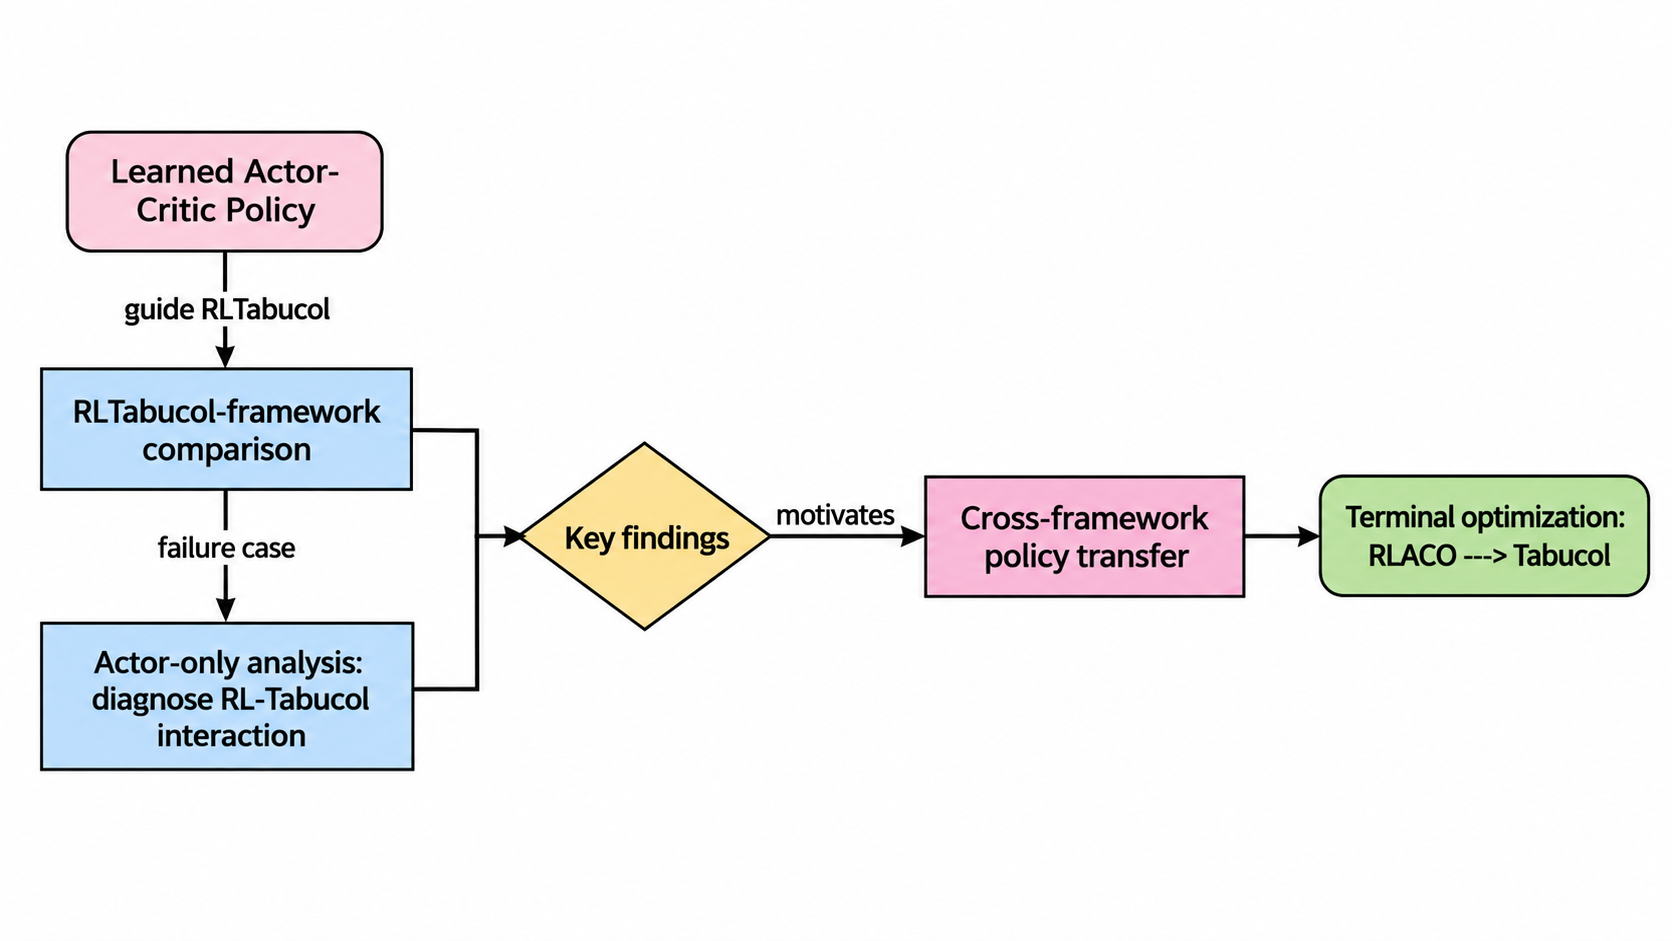
\includegraphics[width=\linewidth]{../figures/method_overview.png}
\caption{Overview of the methodology. A single actor--critic policy is trained in the source RLTabucol setting, frozen, and then evaluated through source-framework comparison, actor-only diagnosis, cross-framework transfer to ACO, and terminal RLACO$\rightarrow$Tabucol optimization.}
\label{fig:method-overview}
\end{figure*}

\subsection{Learned Actor-Critic policy}
\label{ssec:policy}

The shared learned policy selects vertex--color recoloring actions. We model each RL phase as a finite-horizon Markov decision process consisting of \(I\) sequential recoloring steps. At step $t$, the state contains the graph $G=(V,E)$, the color budget $k$, and the current coloring $c_t$. An action is a vertex--color pair $a_t=(v_t,q_t)$ specifying the vertex to recolor and its target color. The immediate reward at RL step $t$ is the reduction in the number of
conflicting edges caused by the recoloring:
\begin{equation}
r_t^{\mathrm{imm}}
=
f(c_{t-1})-f(c_t),
\label{eq:immediate-reward}
\end{equation}
where $f(c)$ denotes the number of conflicting edges in coloring $c$.
Thus, a positive reward indicates conflict reduction, zero indicates no
change, and a negative reward indicates an increase in conflicts. After the final RL step, the resulting coloring $c_I$ is passed to
Tabucol. If $c^{\mathrm{ret}}$ is the coloring returned by Tabucol, the
downstream reward is
\begin{equation}
r_{\mathrm{Tabu}}
=
f(c_I)-f(c^{\mathrm{ret}}).
\label{eq:tabu-reward}
\end{equation}

The reward used for the RL transition is therefore
\begin{equation}
r_t
=
r_t^{\mathrm{imm}}
+
\mathbb{I}[t=I]\,r_{\mathrm{Tabu}},
\label{eq:total-reward}
\end{equation}
where $\mathbb{I}[t=I]$ is one only for the final RL transition and zero
otherwise. With $I=300$, the first $299$ transitions receive only the
immediate conflict-reduction reward, while the $300$th transition receives
both the immediate reward and the downstream Tabucol reward. Therefore, this  reward is intended to encourage the policy not only to reduce conflicts during the RL phase, but also to favor handoff states that allow Tabucol to make further progress.


The policy is implemented as an actor--critic architecture. The actor network factorizes the joint action distribution into a vertex-selection distribution and a conditional color-selection distribution:
\begin{equation}
  \pi_{\theta,\phi}((v,q)\mid s)
  =
  \pi^{\mathrm{v}}_\theta(v\mid s)\,
  \pi^{\mathrm{c}}_\phi(q\mid s,v).
  \label{eq:rl_policy_factorisation}
\end{equation}
The vertex-selection head $\pi^{\mathrm{v}}_\theta$ is a two-layer multilayer perceptron ($3\!\to\!16\!\to\!1$ with ReLU) applied independently to each vertex, followed by a softmax over vertices. It uses three vertex-level features: degree, conflicting-edge count, and number of distinct neighbor colors. The color-selection head $\pi^{\mathrm{c}}_\phi$ is a separate two-layer MLP with the same width, applied to each vertex--color pair and followed by a softmax over colors. It uses three color-level features: number of neighbors assigned the candidate color, color-class size, and total vertex count. Because the same MLP is applied independently to every vertex or vertex--color pair, changing the graph size or color budget changes only the number of evaluations, not the actor's parameters, the actor can be evaluated on different graph sizes and color budgets without changing its parameterization.

The critic uses the same feature-processing structure without the actor softmax layers and appends a linear layer over the flattened $n\times k$ representation to estimate the scalar state value $V_\psi(s)$. This value is used to compute advantage estimates for Proximal Policy Optimization (PPO)~\cite{schulman2017ppo}; PPO updates both actor and critic parameters using the standard clipped surrogate objective. We train a single source policy on Erd\H{o}s--R\'enyi
$G(n{=}250,p{=}0.5)$ graphs with $k{=}24$ for $50$ training epochs; this fixed training setting provides
one common source policy for all subsequent experiments. The same policy
is reused without fine-tuning so that differences across the source, transfer,
and terminal experiments reflect how the policy is used in each framework,
rather than differences caused by retraining or selecting different policies. Detailed PPO and training parameters are reported in Appendix~\ref{app:experimental-details}.

\subsection{RLTabucol source framework}
\label{ssec:rltabucol}

We implement RLTabucol by interleaving the learned policy with Tabucol local search within an episodic loop~\cite{cai2019rlho,frijters2023rltabucol}. Each run starts from a random $k$-coloring. 

Within each episode, the actor performs $I$ sequential recoloring steps, producing an intermediate coloring that is then passed to Tabucol. Tabucol is a single-solution local search that iteratively selects the best admissible vertex recoloring, subject to a tabu list that prevents recently reversed moves. Within RLTabucol, Tabucol performs at most $T$ single-vertex recoloring iterations and returns both a coloring and the reward in Eq.~\eqref{eq:tabu-reward}. The detailed Tabucol procedure is given in Algorithm~\ref{alg:tabucol} in Appendix~\ref{app:experimental-details}.

The returned coloring becomes the starting state of the next episode. With probability $\beta$, Tabucol returns its current coloring; with probability $1-\beta$, it returns the best coloring found during Tabucol phase. The best coloring is therefore retained most of the time, while occasionally
returning the current coloring allows the next RL episode to continue from a
different state rather than always from the local best.  RLTabucol therefore follows one continuing sequence of RL and Tabucol updates rather than restarting independently at every episode. Algorithm~\ref{alg:rltabucol} summarizes the complete pipeline. During training, the collected trajectories are used for PPO updates; during testing, the actor remains fixed.

\begin{algorithm}[t]
\caption{The RLTabucol pipeline}
\label{alg:rltabucol}
\begin{algorithmic}[1]
\State \textbf{Input:} $G$, $k$, actor $\pi_{\theta,\phi}$, steps $I$,
Tabucol iters $T$, prob.\ $\beta$, budget $\mathcal{B}$
\State $c\leftarrow$ random $k$-coloring;\quad $c^\star\leftarrow c$
\While{$\mathcal{B}$ not exhausted}
  \For{$t=0,\dots,I-1$}
    \State $(v,q)\sim\pi_{\theta,\phi}(\cdot\mid(G,k,c))$;\quad $c\leftarrow c[v\mapsto q]$
    \If{$f(c)<f(c^\star)$} \State $c^\star\leftarrow c$ \EndIf
    \If{$f(c^\star)=0$} \State \Return $c^\star$ \EndIf
  \EndFor
  \State $c\leftarrow\textsc{Tabucol}(G,k,c,T,\beta)$
  \If{$f(c)<f(c^\star)$} \State $c^\star\leftarrow c$ \EndIf
  \If{$f(c^\star)=0$} \State \Return $c^\star$ \EndIf
\EndWhile
\State \Return $c^\star$
\end{algorithmic}
\end{algorithm}

Two baselines are used to evaluate RLTabucol. RLTabucol$_0$ replaces the trained actor with a uniform random policy over the same vertex--color action space while keeping the episodic RL--Tabucol structure unchanged; it tests whether the learned actor contributes useful guidance beyond random recoloring. Pure Tabucol uses the same Tabucol implementation and tabu settings as a standalone solver, without any RL guidance, providing a direct baseline for evaluating whether the RLTabucol framework improves over conventional Tabucol and becomes a stronger optimizer. Run counts, time limits, tested color budgets, and evaluation metrics are specified in Section~\ref{ssec:exp-settings}.

\subsection{Actor-only analysis}
\label{ssec:actor-only}

To further diagnose the inconsistent results and investigate the behavior of actor. We design and implement the actor-only diagnostic, which separates the policy's standalone conflict-reduction capability from the downstream repair supplied by Tabucol. Tabucol is disabled while the frozen actor performs the same $I$ recoloring steps, and the conflict trajectory and running-best value are recorded. Comparing this behavior with the full RLTabucol trajectory shows how far the actor can reduce conflicts by itself, how much additional repair is supplied by Tabucol, and whether the remaining difficulty is consistent with the interaction between the two stages rather than the complete failure of either component in isolation. The tested failure case and evaluation protocol are specified in Section~\ref{ssec:exp-settings}.

\subsection{Cross-framework transfer to ACO via soft pheromone injection}
\label{ssec:rlaco}

To test whether the learned policy remains useful when its guidance is consumed by a structurally different search process, we introduce RLACO, which transfers the same policy from the Tabucol-based source framework to ACO through soft pheromone injection. In RLACO, the actor's per-vertex color-selection distribution is mapped to
the initial pheromone matrix, thereby biasing the color choices of the ants.
Each ant then constructs a complete coloring from scratch under this soft
policy guidance. Thus, the transferred information is the policy's learned
color preference rather than a prescribed coloring, allowing the same frozen policy to guide multiple ACO constructions without retraining.

The ACO component follows a MAX--MIN ant system~\cite{stutzle2000maxmin} with pheromone clipping, elite reinforcement, and a pseudo-random-proportional construction rule. Each ant constructs a complete coloring by visiting vertices one by one and selecting colors from the combination of pheromone and heuristic information. The detailed ACO procedure is given in Algorithm~\ref{alg:aco} in Appendix~\ref{app:experimental-details}.

The key interface is soft pheromone injection. Given the current state $s$, the actor's color-selection head produces
$P(v,q)=\pi^{\mathrm{c}}_\phi(q\mid s,v)$, with
$\sum_{q=1}^{k}P(v,q)=1$, representing the preference for assigning color $q$ to vertex $v$. At the end of each RL phase, before the corresponding ACO call, the pheromone matrix is reset to the uniform base level $\tau_0$ and the policy distribution is injected as
\begin{equation}
  \tau(v,q)
  \leftarrow
  \tau_0 +
  \bigl(\min(\tau_{\max},\, \sigma\tau_0) - \tau_0\bigr)\,
  P(v,q),
  \label{eq:soft}
\end{equation}
where $\sigma>1$ is the injection strength. The resulting pheromone values are clipped to $[\tau_{\min},\tau_{\max}]$. The actor provides a soft pheromone prior rather than a deterministic
coloring: each ant still constructs a complete coloring from scratch under
the biased pheromone. The coloring produced by the preceding RL phase is
retained separately as the initial ACO incumbent, while each ant still constructs a coloring from scratch under the biased
pheromone. Standard ACO evaporation and elite reinforcement then update
pheromone during the construction process.
Thus, the RL phase influences ACO through both the soft
pheromone bias and the initial incumbent. Algorithm~\ref{alg:rlaco} summarizes the transfer pipeline.

\begin{algorithm}[t]
\caption{The RLACO pipeline}
\label{alg:rlaco}
\begin{algorithmic}[1]
\State \textbf{Input:} $G$, $k$, actor $\pi_{\theta,\phi}$, steps $I$,
ACO iters $T_{\mathrm{ACO}}$, ants $m$, budget $B$
\State \textbf{Params:} $\tau_0,\tau_{\min},\tau_{\max},\sigma$
\State $c\leftarrow$ random $k$-coloring;\quad $c^\star\leftarrow c$
\While{elapsed $<B$}
  \For{$t=0,\dots,I-1$}
    \State $(v,q)\sim\pi_{\theta,\phi}(\cdot\mid s(c))$;\quad $c\leftarrow c[v\mapsto q]$
    \If{$f(c)<f(c^\star)$} \State $c^\star\leftarrow c$ \EndIf
  \EndFor
  \State $P(v,q)\leftarrow\pi^{\mathrm{c}}_\phi(q\mid s(c),v)$
  \State $\tau\leftarrow\textsc{SoftInject}(P,\tau_0,\tau_{\min},\tau_{\max},\sigma)$
  \State $c\leftarrow\textsc{ACO}(G,k,c,\tau,m,T_{\mathrm{ACO}})$
  \If{$f(c)<f(c^\star)$} \State $c^\star\leftarrow c$ \EndIf
  \If{$f(c^\star)=0$} \State \Return $c^\star$ \EndIf
\EndWhile
\State \Return $c^\star$
\end{algorithmic}
\end{algorithm}

To evaluate the transferred guidance, we compare RLACO$_{\rm soft}$ with three reference configurations: Pure ACO, the random-policy transfer reference RLACO$0$, and the structured conflict-prior configuration RLACO${\rm config}$.  RLACO$_0$ replaces the trained actor with a random policy while preserving the same RL-step and ACO structure. Since the random policy has no learned per-vertex distribution, its realized random-policy coloring is used to bias pheromone toward the vertex--color assignments present in that coloring; RLACO$_0$ is therefore a random-policy transfer reference rather than a perfectly matched soft-prior ablation. Pure ACO removes the RL phase and runs the same ACO continuously without external policy guidance; its pheromone state is retained throughout the run rather than reinitialized between successive ACO calls. RLACO$_{\rm config}$ retains the trained RL phase and the soft-injection mechanism but replaces the learned distribution with a structured conflict-based pheromone prior,
Let $H_v(s,q)$ denote the number of neighbors of vertex $v$ assigned
color $q$ in the complete post-RL coloring represented by state $s$.
The structured conflict-based pheromone prior is defined as
\begin{equation}
 P_{\mathrm{conf}}(v,q)
 =
 \frac{(1+H_v(s,q))^{-1}}
 {\sum_{r=1}^{k}(1+H_v(s,r))^{-1}},
 \label{eq:conf-prior}
\end{equation}
which assigns higher prior probability to colors that currently appear
less frequently among the neighbors of $v$. This baseline replaces the
learned color-selection distribution with a state-dependent structured
conflict-based prior while keeping the trained RL phase and the same
soft-injection pipeline unchanged. ACO local-search post-processing is disabled in RLACO, RLACO$_0$, RLACO$_{\rm config}$, and Pure ACO. This isolates transfer through the ACO construction process: adding local repair at this stage would mix the quality of the transferred guidance with the effect of a downstream local solver. The terminal experiment in Section~\ref{ssec:terminal-method} evaluates that complete optimization question separately.

To examine how the transferred guidance is used inside RLACO, we record the conflict count at three checkpoints in each episode: before the RL phase ($f_e^{\mathrm{start}}$), after the RL phase ($f_e^{\mathrm{RL}}$), and after ACO ($f_e^{\mathrm{ACO}}$). The positive conflict reduction attributed descriptively to each phase is
\begin{align}
  \Delta_e^{\mathrm{RL}}
  &=
  \bigl[f_e^{\mathrm{start}} - f_e^{\mathrm{RL}}\bigr]_+,
  &
  \Delta_e^{\mathrm{ACO}}
  &=
  \bigl[f_e^{\mathrm{RL}} - f_e^{\mathrm{ACO}}\bigr]_+,
\end{align}
where $[x]_+=\max(x,0)$ assigns zero positive reduction to a phase that increases conflicts. Aggregating over episodes gives $S_{\mathrm{RL}}$ and $S_{\mathrm{ACO}}$, with
\begin{equation}
  \mathrm{share}^{\mathrm{RL}}
  =
  \frac{S_{\mathrm{RL}}}
       {S_{\mathrm{RL}}+S_{\mathrm{ACO}}},
  \qquad
  \mathrm{share}^{\mathrm{ACO}}
  = 1 - \mathrm{share}^{\mathrm{RL}}.
  \label{eq:phase-share}
\end{equation}
Because ACO acts on the state produced by the preceding RL phase, these shares are descriptive rather than causal. They distinguish whether positive conflict reduction is recorded mainly during the RL phase or during the subsequent ACO construction phase.

\subsection{RLACO$\rightarrow$Tabucol terminal optimization}
\label{ssec:terminal-method}

The terminal RLACO$\rightarrow$Tabucol experiment tests whether the best coloring found by RLACO can provide a stronger starting point for Tabucol and thereby improve final graph-coloring performance to achieve the goal of optimization. We use the soft-injection RLACO configuration to construct an initialization, then pass its best coloring to downstream Tabucol run using the same Tabucol implementation as the Pure Tabucol baseline and no additional RL phase. Thus, We proposed a framework called RLACO$\rightarrow$Tabucol.


\section{Experimental Setup}
\label{sec:setup}

\subsection{Benchmark instances}
\label{ssec:instances}

The experiments are conducted on instances from the DIMACS graph
coloring benchmark suite. These instances are widely used for
evaluating graph coloring algorithms and cover several graph families.
The DSJC instances are random graphs, where the suffix indicates the
edge density. The \texttt{le450} instances are Leighton graphs with
structured coloring constraints. The flat instances are quasi-random
graphs generated with a prescribed target number of colors and
relatively balanced vertex degrees. Table~\ref{tab:instances} lists
the benchmark instances used in the experiments. The second column
reports the pair $\chi/k^\star$, where $\chi$ denotes the chromatic
number when it is known (``?'' indicates that it is unknown) and
$k^\star$ is the number of colors in the best known solution.

\begin{table}[t]
\centering
\caption{DIMACS benchmark instances used in the experiments. Notice the size group is based on the number of vertices: Small for
$n\leq 300$, Medium for $300<n\leq 500$, and Large for $n>500$.}
\label{tab:instances}
\small
\setlength{\tabcolsep}{5pt}
\begin{tabular}{@{}lccrl@{}}
\toprule
Instance & $\chi/k^\star$ & Size & $n$ & Family \\
\midrule
\texttt{DSJC250.5}        & ?/28   & Small  & 250  & Random, density 0.5 \\
\texttt{DSJC500.1}        & ?/12   & Medium & 500  & Random, density 0.1 \\
\texttt{DSJC500.5}        & ?/47   & Medium & 500  & Random, density 0.5 \\
\texttt{DSJC500.9}        & ?/126  & Medium & 500  & Random, density 0.9 \\
\texttt{flat300\_26\_0}   & 26/26  & Small  & 300  & Flat graph \\
\texttt{flat300\_28\_0}   & 28/28  & Small  & 300  & Flat graph \\
\texttt{flat1000\_76\_0}  & 76/81  & Large  & 1000 & Flat graph \\
\texttt{le450\_15c}       & 15/15  & Medium & 450  & Leighton graph \\
\texttt{le450\_15d}       & 15/15  & Medium & 450  & Leighton graph \\
\texttt{le450\_25c}       & 25/25  & Medium & 450  & Leighton graph \\
\texttt{le450\_25d}       & 25/25  & Medium & 450  & Leighton graph \\
\bottomrule
\end{tabular}
\end{table}

\subsection{Experimental settings and evaluation metrics}
\label{ssec:exp-settings}

Detailed parameter settings for RLTabucol, RLACO, and PPO are reported
in Appendix~A. Training is performed only on Erd\H{o}s--R\'enyi random
graphs using a T4 GPU; no DIMACS instance is used during training.
Testing is conducted on CPU, and all reported times are wall-clock times.
Unless stated otherwise, each experimental configuration is evaluated
with ten independent runs.

For the RLTabucol-related framework experiment, RLTabucol, RLTabucol$_0$, and
Pure Tabucol are evaluated on the same tested color budgets with a
five-hour ($18{,}000$\,s) time limit per run. The five-hour time limit follows the source RLTabucol evaluation protocol
and is consistent with long run-time budgets used in previous DIMACS
graph-coloring studies~\cite{frijters2023rltabucol,zhou2018plscoll}. The primary metric
is $k_{\mathrm{best}}$, the smallest tested color budget for which a
legal coloring ($f(c)=0$) is found. At the same $k$, success count and
successful-run time are used as secondary measures. Success denotes
the number of zero-conflict runs out of ten; time is reported as the
best and mean wall-clock time over successful runs only. The actor-only
diagnostic uses the same five-hour protocol on
typical failure case, with the final running-best conflict
values summarized by their range, mean, and median.

For the cross-framework transfer experiment, RLACO$_{\rm soft}$,
RLACO$_0$, RLACO$_{\rm config}$, and Pure ACO are evaluated at the
fixed target color budgets listed in Table~\ref{tab:rlaco-config}.
\texttt{flat1000\_76\_0} is excluded from the transfer experiment because its 1000-vertex size makes each ACO construction substantially more
expensive, resulting in too few completed ACO calls within a practical
wall-clock budget for a stable fixed-$k$ transfer comparison. Each instance uses an instance-specific wall-clock budget determined from preliminary RLACO runs to provide sufficient time for the running-best conflict value to stabilize. Stabilization is assessed by the relative improvement over the final 10% of the allocated budget, which is negligible across the tested instances.  The same instance-specific budget is then applied to
RLACO$_{\rm soft}$, RLACO$_0$, Pure ACO, and RLACO$_{\rm config}$ on that
instance. The main metric is the final running-best conflict
value at the fixed target $k$, reported as the observed best and
mean$\pm$sample standard deviation over ten runs. For the primary
RLACO$_{\rm soft}$--RLACO$_0$ comparison, two-sided Welch
two-sample $t$-tests are applied to the ten final conflict values, with
Holm correction across the ten instances. The phase-contribution
analysis is computed from the same RLACO$_{\rm soft}$ runs using
Eq.~\eqref{eq:phase-share}.

Finally, the RLACO$\rightarrow$Tabucol experiment uses the same
instance-specific RLACO preparation budget as the corresponding
transfer experiment, followed by the same five-hour downstream
Tabucol run. It also uses the same evaluation  as the
source-framework experiment: $k_{\mathrm{best}}$ is the primary metric,
with success count and best/mean successful-run time used as secondary
measures at comparable color budgets. For
RLACO$\rightarrow$Tabucol, the reported solving time starts when the
prepared coloring is handed to Tabucol; the preceding RLACO
preparation time is not included in this downstream timing measure because the timing measure is intended to evaluate
downstream Tabucol refinement from the RLACO-produced initialization.


\section{Results}
\label{sec:results}

\subsection{Effectiveness of the learned policy: RLTabucol vs. RLTabucol$_0$ and Pure Tabucol}
\label{ssec:res-default}

Table 2 compares RLTabucol with its random-policy baseline RLTabucol$_0$ and standalone Pure Tabucol. Against the matched random-policy control RLTabucol$_0$, RLTabucol matches or improves the achieved $k_{\mathrm{best}}$ on 8 of 11 instances: it reaches a lower $k_{\mathrm{best}}$ on four, ties on four, and requires one additional color on three. The largest reductions are two colors on \texttt{DSJC500.9} and three colors on \texttt{flat1000\_76\_0}. At the same time, the three failures show that the learned guidance is not uniformly beneficial. The policy is therefore clearly different from random recoloring and proved useful, but its value is non-universal across test instances

The comparison with Pure Tabucol tests more directly whether adding the learned policy improves the final graph-coloring solution quality over traditional Tabucol to achieve the goal of optimization. Both methods receive the same five-hour wall-clock budget. However, pure Tabucol spends this budget entirely on local search, whereas RLTabucol divides it between actor inference and repeated Tabucol calls. RLTabucol lowers $k_{\mathrm{best}}$ only on \texttt{flat1000\_76\_0} ($87$ versus $88$), ties Pure Tabucol on nine instances, and is worse on \texttt{flat300\_28\_0} ($31$ versus $30$). At tied color budgets, timing and success are also mixed. On \texttt{DSJC500.1}, for example, RLTabucol reaches $k=12$ in $8/10$ runs and has a lower best and mean successful-run time than Pure Tabucol, whereas on \texttt{DSJC500.5} it succeeds in only $6/10$ runs at $k=49$, compared with $10/10$ for Pure Tabucol. Thus, RLTabucol shows that the learned policy can be useful, but the RLTabucol framework does not yet consistently surpass Pure Tabucol and therefore does not fully realize the intended optimization objective.

Taken together, the first between RLTabucol and RLTabucol$_0$ establishes that the learned policy carries useful search information, whereas the second comprison between RLTabucol and pure tabucol shows that RLTabucol itself is not yet a consistently stronger optimizer than Pure Tabucol. To further investigate the failure cases and the behavior of policy, the actor-only experiment in the next section therefore examines what the policy can achieve without Tabucol, how much fine repair Tabucol contributes, and whether their handoff is a plausible source of the remaining limitation.

\begin{table*}[t]
\centering
\caption{Comparison among Pure Tabucol, RLTabucol, and the random-policy baseline RLTabucol$_0$. Time reports best / mean wall-clock seconds over successful runs only. Bold $k_{\rm best}$ values are the lowest per row, including ties. Best and mean times are compared and bolded independently only among methods attaining the row-minimum color budget.}
\label{tab:rltabucol-default}
\setlength{\tabcolsep}{2.5pt}
\resizebox{\textwidth}{!}{\begin{tabular}{@{}lccccccccc@{}}
\toprule
Instance & \multicolumn{3}{c}{Pure Tabucol} & \multicolumn{3}{c}{RLTabucol} & \multicolumn{3}{c}{RLTabucol$_0$}\\
 & $k_{\rm best}$ & Success & Time (s) & $k_{\rm best}$ & Success & Time (s) & $k_{\rm best}$ & Success & Time (s)\\
\midrule
\texttt{DSJC250.5} & \textbf{28} & 10/10 & 14.6 / 45.5 & \textbf{28} & 10/10 & 243.8 / 3046.5 & \textbf{28} & 10/10 & \textbf{2.6} / \textbf{269.0} \\
\texttt{DSJC500.1} & \textbf{12} & 7/10 & 2356.2 / 6001.4 & \textbf{12} & 8/10 & \textbf{936.9} / \textbf{3616.9} & 13 & 10/10 & 0.4 / 0.6 \\
\texttt{DSJC500.5} & \textbf{49} & 10/10 & \textbf{408.5} / \textbf{1519.6} & \textbf{49} & 6/10 & 2375.5 / 7664.3 & 50 & 10/10 & 101.9 / 1303.2 \\
\texttt{DSJC500.9} & \textbf{128} & 8/10 & \textbf{2513.0} / \textbf{8521.6} & \textbf{128} & 4/10 & 3062.7 / 8749.3 & 130 & 7/10 & 1080.5 / 4289.1 \\
\texttt{le450\_15c} & 16 & 10/10 & 0.2 / 45.2 & 16 & 10/10 & 4.1 / 246.7 & \textbf{15} & 10/10 & \textbf{273.1} / \textbf{1283.2} \\
\texttt{le450\_15d} & 16 & 9/10 & 0.3 / 302.5 & 16 & 10/10 & 32.2 / 1085.3 & \textbf{15} & 9/10 & \textbf{932.4} / \textbf{6956.8} \\
\texttt{le450\_25c} & \textbf{26} & 9/10 & 5.4 / 12.4 & \textbf{26} & 10/10 & 44.7 / 141.0 & \textbf{26} & 10/10 & \textbf{3.3} / \textbf{16.5} \\
\texttt{le450\_25d} & \textbf{26} & 10/10 & 7.6 / 14.5 & \textbf{26} & 10/10 & 44.8 / 106.6 & \textbf{26} & 10/10 & \textbf{1.9} / \textbf{17.5} \\
\texttt{flat300\_26\_0} & \textbf{26} & 10/10 & \textbf{8.8} / \textbf{215.8} & \textbf{26} & 10/10 & 229.2 / 1147.8 & \textbf{26} & 10/10 & 134.3 / 704.4 \\
\texttt{flat300\_28\_0} & \textbf{30} & 1/10 & \textbf{9453.8} / \textbf{9453.8} & 31 & 10/10 & 150.4 / 1278.2 & \textbf{30} & 1/10 & 14021.1 / 14021.1 \\
\texttt{flat1000\_76\_0} & 88 & 1/10 & 16485.4 / 16485.4 & \textbf{87} & 1/10 & \textbf{8920.2} / \textbf{8920.2} & 90 & 10/10 & 303.9 / 1349.2 \\
\bottomrule
\end{tabular}
}
\end{table*}

\subsection{Actor-only analysis of the policy--Tabucol interface}
\label{ssec:res-actor}

We select \texttt{le450\_15d} as a representative failure case and examine
the actor's standalone behavior at $k=15$ in
Figure~\ref{fig:actor-only-curve}. Across ten complete actor-only runs, the best conflict counts at termination range from $203$ to $243$, with mean $225.5$ and median $223.5$. The ten complete diagnostic runs finish between $5$ and $21$ conflicts, with mean $12.7$ and median $13.5$ (rounded to $14$ in the figure). Removing Tabucol leaves the actor with 203--243 residual conflicts,
whereas the full RLTabucol pipeline reduces the final conflict count to
5--21. This large gap shows that the actor provides useful coarse
conflict reduction but relies on Tabucol for most of the fine-grained
repair. Nevertheless, none of the full-pipeline runs reaches zero
conflicts, indicating that the combination still fails to complete the
final repair on this instance.

These observations rule out the simple explanations that the actor
provides no useful guidance or that Tabucol contributes little to the
search. Instead, they point to the actor--Tabucol interaction as a
plausible limitation: the actor can produce lower-conflict states, and
Tabucol can substantially refine them, yet the resulting trajectory does
not consistently reach a state from which the remaining conflicts can be
eliminated. This is consistent with a mismatch between minimizing the
current conflict count and producing handoff states that are favorable
for subsequent Tabucol repair.

This interpretation may be consistent with the training signal described in Section~\ref{ssec:policy}. Immediate conflict reduction is rewarded throughout the $300$-step RL phase, whereas information about Tabucol's response enters only at the final transition. This delayed downstream feedback may make it easier for the actor to learn how to reach low-conflict states than to distinguish which low-conflict states are easiest for Tabucol to repair. Because each episode starts from the coloring returned by the previous one, successive handoff states may remain closely related, potentially limiting the range of starting states presented to Tabucol.

Overall, these observations suggest that useful conflict reduction by the actor does
not necessarily translate into a favorable handoff for final Tabucol repair.
We therefore test whether the same frozen policy remains useful under a
different search interface by transferring its learned color preferences to
ACO, where they bias multiple alternative constructions rather than a single
directly repaired coloring. Moreover, if the transferred guidance remains useful in ACO,
the resulting best incumbent can then be evaluated as an initialization for a
separate downstream Tabucol stage.

\begin{figure}[t]
\centering
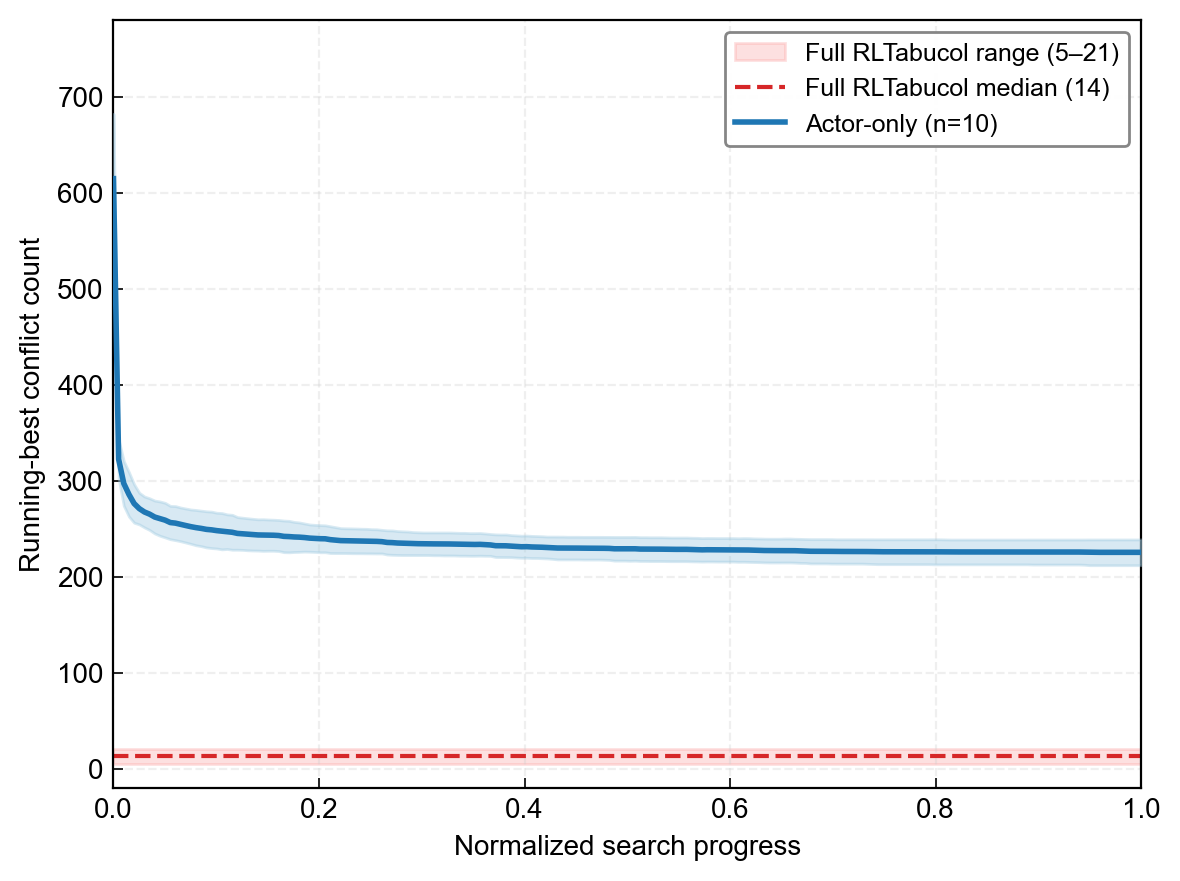
\includegraphics[width=\linewidth]{../figures/generated/actor_only_le45015d.png}
\caption{Actor-only diagnostic on \texttt{le450\_15d} ($k=15$). The actor-only curve summarizes ten runs over normalized search progress; the red band shows the full RLTabucol final range of $5$--$21$ conflicts. Its median of $13.5$ is rounded to $14$ in the legend.}
\label{fig:actor-only-curve}
\end{figure}

\subsection{Cross-framework policy transfer}
\label{ssec:res-rlaco}

Motivated by the actor-only analysis, we next test whether the same frozen policy is more useful when its guidance is consumed by a population-based constructor rather than handed directly to Tabucol. Table~\ref{tab:rlaco-config} reports the results: RLACO$_{\rm soft}$ obtains lower observed best and mean conflicts than both Pure ACO and RLACO$_0$ on all ten instances. Relative to RLACO$_0$, the observed-best reduction ranges from $20$ conflicts on \texttt{le450\_25c} to $154$ on \texttt{DSJC500.9}. Two-sided Welch tests on the ten final conflict values per configuration remain significant after Holm correction on all ten instances, with a largest adjusted $p$-value of $0.00122$. The three source-framework failure cases are particularly informative.
Relative to RLACO$_0$, RLACO$_{\rm soft}$ reduces the observed best from
$150$ to $58$ on \texttt{flat300\_28\_0}, from $295$ to $222$ on
\texttt{le450\_15c}, and from $290$ to $229$ on \texttt{le450\_15d}.
These values remain nonzero, so the transfer stage does not recover legal
colorings at the tested color budgets. Nevertheless, the same frozen policy
that underperforms random guidance on these instances in the source
RLTabucol framework yields lower residual conflicts than RLACO$_0$ when
its learned preferences are used to guide ACO. Overall, these results suggest that policy
usefulness depends not only on the learned guidance itself, but also on how
that guidance is used by the surrounding search framework.

The comparison with RLACO$_{\rm config}$ focuses more directly on the transferred prior. RLACO$_{\rm soft}$ achieves a lower observed best on six instances, ties on \texttt{DSJC500.9}, and is worse on three. Two of the three losses are only one conflict, on \texttt{flat300\_28\_0} and \texttt{le450\_15c}. On the tied \texttt{DSJC500.9} case, RLACO$_{\rm soft}$ also has a lower mean and standard deviation ($47.4\pm3.4$ versus $48.4\pm3.9$). In the other direction, the learned prior improves the observed best by $17$ conflicts on both \texttt{le450\_25c} ($43$ versus $60$) and \texttt{le450\_25d} ($44$ versus $61$), and by $9$ on \texttt{DSJC500.1} ($48$ versus $57$). Although it does not win on every instance, the learned prior is stronger overall than the conflict-constructed prior: it wins more often than it loses, and several of its gains are substantially larger than its small losses.

\begin{table*}[t]
\centering
\caption{Transfer comparison at fixed tested $k$. Entries are best conflicts (mean$\pm$sample standard deviation); the lowest best value per row is bold, including ties. All cells contain ten complete runs. RLACO$_0$ is the random-policy transfer reference defined in Section~\ref{ssec:rlaco}. Welch $t$ uses RLACO$_0$ minus RLACO$_{\rm soft}$, with ten runs per group; two-sided $p$-values are Holm-adjusted across ten instances.}
\label{tab:rlaco-config}
\setlength{\tabcolsep}{3pt}
\resizebox{\textwidth}{!}{\begin{tabular}{@{}lccccccc@{}}
\toprule
Instance & $\chi/k^\star$ & $k$ & Pure ACO & RLACO$_0$ (hard) & RLACO$_{\rm config}$ & RLACO$_{\rm soft}$ & Welch $t$\\
\midrule
\texttt{DSJC250.5} & ?/28 & 28 & 69 (74.6$\pm$3.5) & 70 (76.6$\pm$2.9) & 21 (24.7$\pm$2.8) & \textbf{16 (22.7$\pm$3.1)} & 39.7 \\
\texttt{DSJC500.1} & ?/12 & 12 & 123 (134.2$\pm$6.1) & 136 (141.4$\pm$2.3) & 57 (65.7$\pm$6.9) & \textbf{48 (62.9$\pm$11.6)} & 21.0 \\
\texttt{DSJC500.5} & ?/47 & 48 & 224 (229.9$\pm$3.1) & 225 (230.0$\pm$3.6) & 76 (84.7$\pm$6.9) & \textbf{74 (78.1$\pm$3.4)} & 97.9 \\
\texttt{DSJC500.9} & ?/126 & 126 & 192 (194.9$\pm$2.8) & 196 (202.1$\pm$3.0) & \textbf{42 (48.4$\pm$3.9)} & \textbf{42 (47.4$\pm$3.4)} & 110.3 \\
\texttt{flat300\_26\_0} & 26/26 & 26 & 179 (187.8$\pm$5.0) & 187 (194.7$\pm$3.6) & \textbf{86 (92.9$\pm$4.9)} & 93 (96.7$\pm$4.9) & 50.9 \\
\texttt{flat300\_28\_0} & 28/28 & 28 & 136 (145.5$\pm$4.8) & 150 (155.6$\pm$2.6) & \textbf{57 (62.3$\pm$4.1)} & 58 (62.4$\pm$3.1) & 73.4 \\
\texttt{le450\_15c} & 15/15 & 15 & 293 (297.6$\pm$2.4) & 295 (298.0$\pm$1.6) & \textbf{221 (237.0$\pm$10.7)} & 222 (244.0$\pm$13.1) & 24.9 \\
\texttt{le450\_15d} & 15/15 & 15 & 295 (300.8$\pm$2.6) & 290 (301.4$\pm$5.3) & 234 (254.5$\pm$13.6) & \textbf{229 (249.2$\pm$13.2)} & 11.6 \\
\texttt{le450\_25c} & 25/25 & 25 & 68 (70.3$\pm$1.7) & 63 (68.0$\pm$2.7) & 60 (62.9$\pm$2.4) & \textbf{43 (57.2$\pm$6.9)} & 4.7 \\
\texttt{le450\_25d} & 25/25 & 25 & 70 (72.2$\pm$1.4) & 66 (70.0$\pm$1.7) & 61 (64.7$\pm$2.4) & \textbf{44 (50.5$\pm$6.4)} & 9.2 \\
\bottomrule
\end{tabular}
}
\end{table*}

To examine how the transferred guidance is used inside RLACO, Figure~\ref{fig:rl_aco_share} reports the positive conflict reduction recorded in the RL and ACO phases. On the random and flat graphs, the RL phase accounts for $91.2\%$--$99.3\%$ of the cumulative positive reduction, while the shares on \texttt{le450\_15c} and \texttt{le450\_15d} fall to $72.1\%$ and $66.7\%$. The pattern changes sharply on \texttt{le450\_25c} and \texttt{le450\_25d}, where the RL shares are only $0.45\%$ and $0.84\%$, yet RLACO$_{\rm soft}$ still gives the strongest observed transfer results on those instances. This is important because it shows that the policy's useful behavior is not limited to conflicts removed directly during the RL phase. On some graphs the policy acts mainly as a direct reducer; On other instances, the policy's color distribution mainly acts as a construction bias, helping ACO generate lower-conflict candidate colorings. This pattern also indicates that the policy's utility is not limited to conflicts
removed directly during the RL phase; its learned color preferences can also
provide useful search bias to the subsequent ACO construction.

Overall, the soft-injection interface transfers useful policy information across frameworks. It consistently improves on unguided and random-policy ACO, is stronger overall than the explicit conflict-constructed prior, and remains useful even when the RL phase itself contributes little direct conflict reduction. These results motivate retaining the learned soft prior for the terminal optimization experiment.

\begin{figure*}[t]
\centering
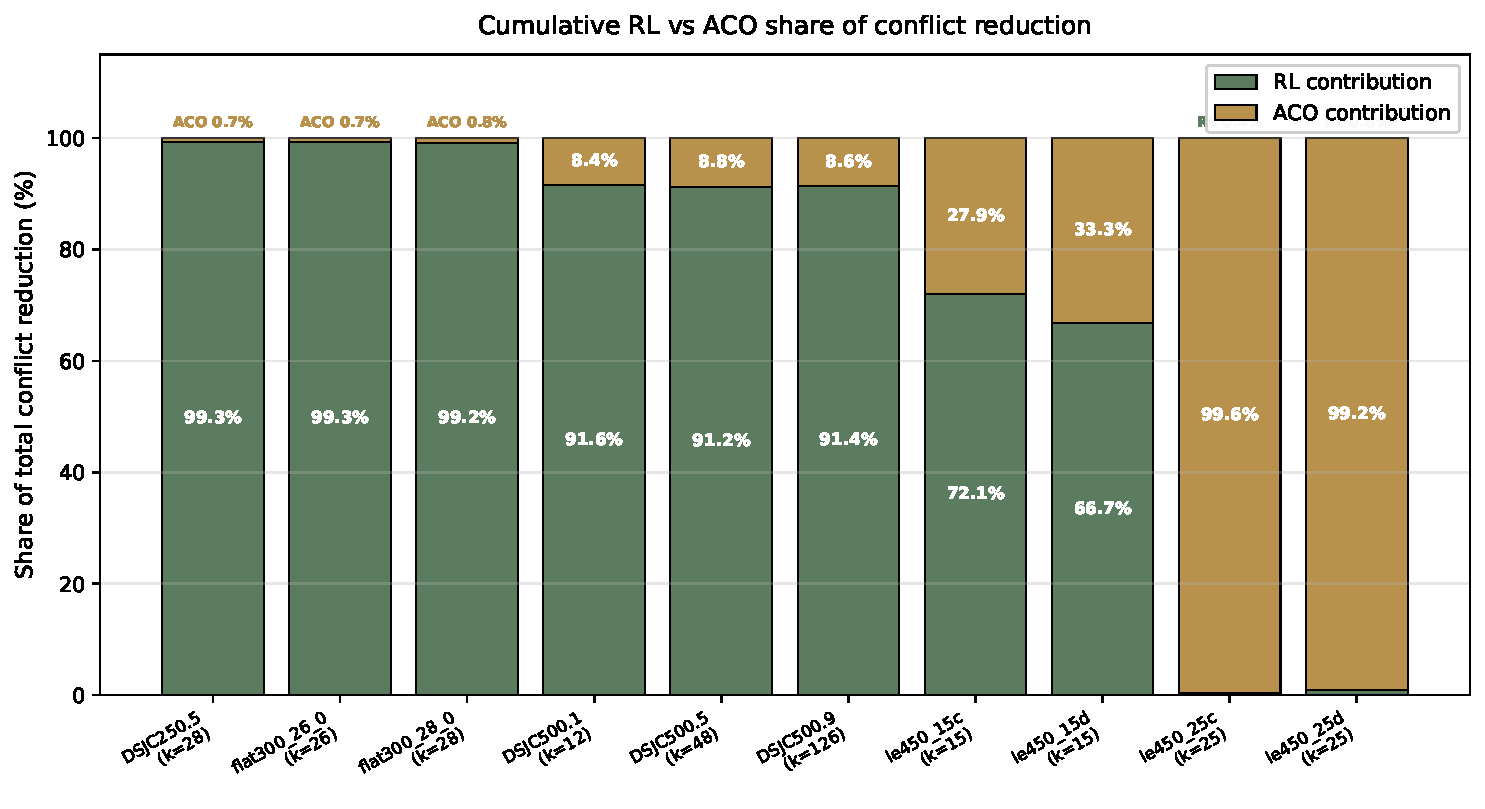
\includegraphics[width=0.85\linewidth]{../figures/generated/component_analysis_vertical.pdf}
\caption{Cumulative shares of positive conflict reduction recorded during the RL and ACO phases across ten transfer instances. The phase-share metric is defined in Section~\ref{ssec:rlaco}.}
\label{fig:rl_aco_share}
\end{figure*}

\subsection{Optimization with RLACO-initialized Tabucol}
\label{ssec:terminal}

The transfer results show that the learned soft prior improves ACO even when the source RLTabucol coupling is inconsistent. We therefore make one final step: use RLACO to prepare the starting coloring for the downstream Tabucol local solver. In RLACO$\rightarrow$Tabucol, the RLACO stage uses the same instance-specific preparation budget as in Section~\ref{ssec:res-rlaco}; its best coloring is then handed to the same Tabucol solver used in the Pure Tabucol baseline. As defined in Section~\ref{ssec:terminal-method}, the reported time starts at this handoff because the timing experiment measures how efficiently Tabucol exploits the prepared initialization.

The results show that RLACO$\rightarrow$Tabucol improves both attainable solution quality and the downstream Tabucol refinement profile. It reaches a lower $k_{\mathrm{best}}$ than Pure Tabucol on five instances and ties it on the other six. Relative to RLTabucol it again records five wins and six ties, and the same $5$--$6$--$0$ win--tie--loss profile holds against RLTabucol$_0$. RLACO$\rightarrow$Tabucol is therefore best or tied for best on all eleven instances. Two cases are strictly better than all three comparators: \texttt{DSJC500.9}, where it reaches $k=126$ instead of $128$, $128$, and $130$, and \texttt{le450\_25d}, where it reaches $k=25$ instead of $26$ for all three source methods. The three instances on which RLTabucol underperformed RLTabucol$_0$ are all recovered at the terminal stage. On \texttt{le450\_15c} and \texttt{le450\_15d}, RLACO$\rightarrow$Tabucol reaches $k=15$ rather than the RLTabucol value of $16$; on \texttt{flat300\_28\_0}, it reaches $k=30$ rather than $31$. The \texttt{DSJC500.9} result gives the clearest link between transfer and optimization: RLACO$_{\rm soft}$ first reduces the fixed-$k=126$ residual to an observed best of $42$ conflicts without local search, after which the downstream Tabucol stage reaches a legal $126$-coloring. The three source methods reach only $128$, $128$, and $130$ colors.

\begin{table*}[t]
\centering
\caption{Terminal optimization comparison. Each method reports its attained $k_{\rm best}$, the number of successful runs out of ten, and best / mean time in seconds over successful runs only. Bold $k_{\rm best}$ values are the lowest per row, including ties. Best and mean times are compared and bolded independently only among methods attaining that row-minimum color budget; times from methods reported at larger $k$ are shown for completeness but are not used for cross-method speed claims. For RLACO$\rightarrow$Tabucol, timing starts at the RLACO-to-Tabucol handoff.}
\label{tab:terminal-comparison}
\setlength{\tabcolsep}{2.1pt}
\resizebox{\textwidth}{!}{% Time is best / mean over successful runs only.
% NOTE: flat300_26_0 RLTabucol mean is set to 1147.8 to match the source-framework table;
% a legacy terminal-time table contained 772.6 and should be checked against raw logs before submission.
\begin{tabular}{@{}lcccccccccccc@{}}
\toprule
Instance & \multicolumn{3}{c}{Pure Tabucol} & \multicolumn{3}{c}{RLTabucol} & \multicolumn{3}{c}{RLTabucol$_0$} & \multicolumn{3}{c}{RLACO$\rightarrow$Tabucol}\\
 & $k_{\rm best}$ & Success & Time (s) & $k_{\rm best}$ & Success & Time (s) & $k_{\rm best}$ & Success & Time (s) & $k_{\rm best}$ & Success & Time (s)\\
\midrule
\texttt{DSJC250.5} & \textbf{28} & 10/10 & 14.6 / 45.5 & \textbf{28} & 10/10 & 243.8 / 3046.5 & \textbf{28} & 10/10 & 2.6 / 269.0 & \textbf{28} & 9/10 & \textbf{1.5} / \textbf{36.5} \\
\texttt{DSJC500.1} & \textbf{12} & 7/10 & 2356.2 / 6001.4 & \textbf{12} & 8/10 & \textbf{936.9} / \textbf{3616.9} & 13 & 10/10 & 0.4 / 0.6 & \textbf{12} & 9/10 & 1358.0 / 4994.4 \\
\texttt{DSJC500.5} & \textbf{49} & 10/10 & \textbf{408.5} / \textbf{1519.6} & \textbf{49} & 6/10 & 2375.5 / 7664.3 & 50 & 10/10 & 101.9 / 1303.2 & \textbf{49} & 10/10 & 424.0 / 1755.7 \\
\texttt{DSJC500.9} & 128 & 8/10 & 2513.0 / 8521.6 & 128 & 4/10 & 3062.7 / 8749.3 & 130 & 7/10 & 1080.5 / 4289.1 & \textbf{126} & 1/10 & \textbf{7330.6} / \textbf{7330.6} \\
\texttt{le450\_15c} & 16 & 10/10 & 0.2 / 45.2 & 16 & 10/10 & 4.1 / 246.7 & \textbf{15} & 10/10 & 273.1 / 1283.2 & \textbf{15} & 2/10 & \textbf{130.8} / \textbf{252.0} \\
\texttt{le450\_15d} & 16 & 9/10 & 0.3 / 302.5 & 16 & 10/10 & 32.2 / 1085.3 & \textbf{15} & 9/10 & 932.4 / 6956.8 & \textbf{15} & 1/10 & \textbf{578.5} / \textbf{578.5} \\
\texttt{le450\_25c} & \textbf{26} & 9/10 & 5.4 / 12.4 & \textbf{26} & 10/10 & 44.7 / 141.0 & \textbf{26} & 10/10 & 3.3 / 16.5 & \textbf{26} & 10/10 & \textbf{1.5} / \textbf{7.4} \\
\texttt{le450\_25d} & 26 & 10/10 & 7.6 / 14.5 & 26 & 10/10 & 44.8 / 106.6 & 26 & 10/10 & 1.9 / 17.5 & \textbf{25} & 2/10 & \textbf{8480.7} / \textbf{8771.6} \\
\texttt{flat300\_26\_0} & \textbf{26} & 10/10 & \textbf{8.8} / 215.8 & \textbf{26} & 10/10 & 229.2 / 1147.8 & \textbf{26} & 10/10 & 134.3 / 704.4 & \textbf{26} & 10/10 & 13.3 / \textbf{167.9} \\
\texttt{flat300\_28\_0} & \textbf{30} & 1/10 & 9453.8 / 9453.8 & 31 & 10/10 & 150.4 / 1278.2 & \textbf{30} & 1/10 & 14021.1 / 14021.1 & \textbf{30} & 1/10 & \textbf{4788.2} / \textbf{4788.2} \\
\texttt{flat1000\_76\_0} & 88 & 1/10 & 16485.4 / 16485.4 & \textbf{87} & 1/10 & \textbf{8920.2} / \textbf{8920.2} & 90 & 10/10 & 303.9 / 1349.2 & \textbf{87} & 1/10 & 13323.9 / 13323.9 \\
\bottomrule
\end{tabular}
}
\end{table*}

The timing results show that the improved initialization is often easier for the downstream Tabucol solver to exploit. Among methods that attain the row-minimum $k_{\mathrm{best}}$, RLACO$\rightarrow$Tabucol has the shortest best successful-run refinement time on seven of eleven instances and the shortest mean successful-run time on eight. Two of those rows, \texttt{DSJC500.9} and \texttt{le450\_25d}, are cases in which RLACO$\rightarrow$Tabucol alone reaches the best color budget. Excluding them gives a stricter shared-target comparison: RLACO$\rightarrow$Tabucol remains fastest on five of nine instances by best successful time and six of nine by mean successful time. This improvement is not explained simply by handing Tabucol a lower-conflict coloring. The original RLTabucol pipeline already presents Tabucol with states after substantial policy-driven conflict reduction, yet it does not consistently outperform Pure Tabucol; the transfer stage changes how the learned information is organized before the downstream handoff.

Success counts provide a complementary measure of reliability, but they must be interpreted at the color budget being attempted. A lower $k$ defines a harder fixed-$k$ problem, so success rates reported at different color budgets are not directly comparable. At the new frontiers, RLACO$\rightarrow$Tabucol succeeds in $1/10$ runs at $k=126$ on \texttt{DSJC500.9} and at $k=15$ on \texttt{le450\_15d}, and in $2/10$ runs on \texttt{le450\_15c} and \texttt{le450\_25d}. At shared targets the pattern is stronger: on \texttt{DSJC500.1} at $k=12$, it succeeds in $9/10$ runs, compared with $8/10$ for RLTabucol and $7/10$ for Pure Tabucol; on \texttt{DSJC500.5} at $k=49$, it reaches $10/10$, matching Pure Tabucol and exceeding RLTabucol's $6/10$. Because solution quality is determined first by the attained color budget, success rate is treated as a secondary reliability measure rather than the primary measure of optimization performance.

Overall, RLACO$\rightarrow$Tabucol converts the cross-framework transfer result into the intended optimization gain. The staged framework reaches equal or better color quality on every tested instance and, once the RLACO initialization is available, gives the downstream Tabucol solver the strongest overall refinement-time profile. The contribution is therefore not limited to transferring a policy between frameworks: the transferred policy is used to construct an initialization that improves both attainable solution quality and downstream solving efficiency.


\section{Discussion and Limitations}
\label{sec:discussion}

\subsection{Learned policy effectiveness and the RLTabucol framework limitation}
\label{ssec:discussion-source}

The source-framework results address two related questions: whether the policy
has learned useful search information, and whether RLTabucol can convert that
information into stronger optimization performance. RLTabucol differs clearly
from its random-policy control and matches or improves it on most tested
instances, indicating that the actor has learned useful vertex--color guidance.
However, it still fails against RLTabucol$_0$ on several instances, and does not
consistently outperform Pure Tabucol to achieve the goal of optimization. The failures observed against both
baselines therefore motivate the actor-only diagnostic, which examines whether
the remaining limitation comes from the policy itself or from its interaction
with Tabucol.

The actor-only diagnostic suggests that the interaction between RL and Tabucol is an important
part of the problem. The actor substantially reduces conflicts without solving
the selected failure instance, while Tabucol provides most of the subsequent
fine repair; nevertheless, the complete RLTabucol algorithm still fails to achive zero-conflict. This suggests that lowering the number of conflicts greatly does not ensure a successful handoff to Tabucol. The reward structure offers a plausible explanation. The
policy receives dense immediate feedback for conflict reduction throughout the
RL phase, whereas information about Tabucol's downstream response is available
only at the final transition and must be propagated back through discounted
credit assignment. The resulting learning signal therefore could more easily provide much more
direct guidance on how to reduce conflicts than on which low-conflict states are
most favorable for Tabucol to solve the problem. In addition, because the coloring returned by
one RL--Tabucol episode becomes the starting point of the next, the search
continues along a single evolving trajectory rather than repeatedly exploring
independent starting states; this may cause it to revisit similar low-conflict
regions that remain difficult for Tabucol to complete. Although state diversity
and basin quality are not directly measured here, these observations suggest
that effective optimization requires not only reaching low-conflict states but
also producing a better downstream handoff. This motivates transferring the
learned preferences to population-based ACO, where they can bias multiple
alternative constructions instead of passing low-conflict areas that Tabucol still finds challenging to solve.

\subsection{Cross-framework transfer and the role of the learned prior}
\label{ssec:discussion-transfer}

The RLACO results show that the usefulness of the learned policy is not
confined to the source RLTabucol framework. The source-framework failure cases are particularly informative. On these instances, RLTabucol underperforms RLTabucol$0$, yet after the same frozen policy is transferred to ACO, RLACO${\rm soft}$ achieves lower fixed-$k$ conflict values than the random-policy transfer reference. Since the two experiments use different search processes and objectives, this should not be interpreted as a direct performance reversal; rather, it shows that the learned policy can still provide useful guidance under a different transfer interface. More
broadly, the soft-transfer configuration consistently outperforms both unguided
ACO and the random-policy transfer reference, while also showing a stronger
overall profile than the structured conflict-based prior. Taken together, these results confirm that the learned policy can be transferred effectively from RLTabucol to ACO through the soft-injection interface.

Soft injection changes how the learned information is used. In RLTabucol, the
coloring produced by the RL phase is handed directly to Tabucol for local
repair. In RLACO, the actor's per-vertex color preferences are instead injected
as a soft pheromone prior, allowing multiple ants to construct different
policy-biased colorings rather than forcing the next search stage to work from
one policy-produced coloring. This gives RLACO an opportunity to search for a policy-informed coloring that is not only low in conflicts but also more suitable for downstream repair; the terminal RLACO$\rightarrow$Tabucol experiment then tests whether the best coloring found by this process provides a better starting point for Tabucol.

The phase analysis further clarifies this complementary role. On some
instances, most positive conflict reduction is recorded directly during the RL
phase. On \texttt{le450\_25c} and \texttt{le450\_25d}, however, the RL share
is below $1\%$, even though the learned soft prior remains highly effective.
Useful policy behavior therefore cannot be identified only with conflicts
removed directly by RL. The learned distribution can also bias which
colorings ACO constructs and reinforces, so its benefit can emerge through the
ACO construction phase rather than through direct RL conflict reduction. This is particularly relevant to the terminal experiment, because the best coloring produced by RLACO can reflect both direct conflict reduction by RL and the use of learned policy preferences across multiple ACO constructions before it is handed to Tabucol. In this way, RLACO preserves the learned guidance while allowing it to be realized through multiple construction alternatives rather than a single policy-produced coloring. Since the phase shares are descriptive and the ACO phase depends on the state produced by RL, these results support complementary roles for the two phases rather than a causal decomposition of their effects.

\subsection{RLACO$\rightarrow$Tabucol: from transfer to optimization}
\label{ssec:discussion-terminal}

The fixed-$k$ RLACO experiment establishes that policy guidance can transfer across frameworks; the terminal experiment shows that this transfer can be converted into an actual graph-coloring optimization gain and achieve the goal of state-of-the-art results. RLACO$\rightarrow$Tabucol framework reaches the best or tied-best color threshold on all eleven tested instances, and it is strictly better than all three source-framework comparators on \texttt{DSJC500.9} and \texttt{le450\_25d}. It also recovers the source-framework failure cases in which RLTabucol was worse than its random-policy baseline. These results make the terminal configuration the strongest evidence for the practical value of cross-framework transfer: the learned guidance not only helps reduce conflicts, but, through soft injection, also biases ACO toward multiple policy-informed constructions, providing Tabucol with a more useful starting point from which legal colorings can be reached at equal or lower color budgets.

The downstream timing results support the same interpretation. Once the RLACO initialization is available, Tabucol is often able to refine it more quickly at comparable color budgets. This improvement should not be reduced to the observation that RLACO produces low-conflict states. The original RLTabucol pipeline also presents Tabucol with states after substantial policy-driven conflict reduction, yet it does not consistently improve on Pure Tabucol. The terminal results are therefore more consistent with a difference in handoff quality: RLACO reorganizes the learned guidance through population-based construction before local repair is applied. The combination of improved color thresholds and frequent downstream timing gains indicates that the resulting initialization is often more useful to Tabucol than a low conflict count alone would suggest.

The resulting framework highlights a complementary division of labor. The RL policy provides reusable vertex--color preferences, ACO converts those preferences into alternative policy-biased constructions, and Tabucol supplies the final local repair. The contribution is therefore not that one component replaces the others, but that the learned information is transferred through an interface that better matches the strengths of the downstream search. In this staged setting, RLACO$\rightarrow$Tabucol improves attainable solution quality while also providing a strong downstream refinement profile. Success rates remain secondary to the attained color number of solving problem, because success counts at different $k$ values correspond to problems of different difficulty.

\subsection{Limitations}
\label{ssec:discussion-limitations}

Several limitations should be considered when interpreting the results.
First, although RLACO$\rightarrow$Tabucol improves attainable solution
quality and the downstream refinement efficiency of Tabucol, generating
the RLACO initialization requires additional preprocessing time. This
cost is intentionally excluded from the reported terminal solving time,
which measures the downstream Tabucol stage after the handoff. The
timing results should therefore be interpreted as improvements in
downstream refinement efficiency rather than as an end-to-end
wall-clock speed advantage.


Second, the present study does not include a complete set of ablations
for the mechanisms underlying the observed transfer. In particular,
the effects of the reward design, policy choice, and soft-injection
strength have not been isolated systematically. The current experiments
therefore establish the effectiveness of the proposed transfer
configuration, but do not fully determine the contribution of each
design choice.

Third, the empirical scope remains limited. The evaluation uses a
moderate set of DIMACS instances, and Tabucol is the only downstream
local-search solver examined in the terminal optimization stage.
Consequently, the extent to which the observed transfer and handoff
benefits generalize to broader benchmark sets and other local-search
methods remains undetermined.

\section{Conclusion}
\label{sec:conclusion}

We investigated whether a reinforcement-learning policy trained inside
RLTabucol learns guidance that is specific to its source framework or remains
useful when transferred to a structurally different search process. The
source-framework experiments show that the learned policy provides useful
vertex--color guidance relative to random recoloring, but RLTabucol does not
consistently outperform Pure Tabucol. The actor-only diagnostic further shows
that the policy can substantially reduce conflicts while Tabucol supplies most
of the fine repair, suggesting that the remaining limitation lies partly in how
the learned guidance is handed to the downstream solver rather than in the
absence of useful policy behavior.

Motivated by these results, we transferred the same policy to ACO
through a soft pheromone-injection interface. The transferred configuration
consistently improves on both unguided ACO and the random-policy transfer
reference at fixed $k$, and shows a stronger overall profile than the structured
conflict-based pheromone prior. The phase analysis further indicates that policy
utility is not limited to conflicts removed directly during the RL phase: the
learned color preferences can also guide the subsequent ACO construction
process. Soft transfer therefore preserves useful policy information while
allowing multiple policy-informed constructions instead of relying on a single
policy-produced handoff state.

The main optimization result is obtained by
RLACO$\rightarrow$Tabucol. The best coloring produced by the complete RLACO
stage is used to initialize a separate downstream Tabucol solver. This
configuration reaches the best or tied-best $k_{\mathrm{best}}$ on all eleven
tested instances, including two cases in which it reaches a lower color budget
than all three source-framework comparators. It also recovers the three cases
in which RLTabucol underperforms its random-policy baseline. Once the RLACO
initialization is available, Tabucol also shows the strongest overall
downstream refinement-time profile. Taken together, these results show that a
policy trained in one search framework can remain useful in another without
retraining, and that transferring its preferences through a population-based
construction process can convert that reusable guidance into improved final
graph-coloring performance and achieve the state-of-the-art results.

Future work should examine the transfer mechanism more systematically through
ablations of the reward design, learned policy, and soft-injection strength, in
order to identify which components contribute most strongly to transferable
guidance and favorable downstream initialization. The evaluation should also
be extended to larger and more diverse benchmark sets, alternative transfer
frameworks, and different downstream local-search solvers to determine how
broadly the observed transfer behavior generalizes. A further promising
direction is to reconsider the role of RL inside Tabucol itself. Rather than
using the policy only to propose recoloring actions, RL could act as a
trajectory-level monitor that observes the progress of Tabucol and dynamically
adjusts search parameters such as tabu tenure, diversification strength,
restart timing, or other search-control decisions. 

\bibliographystyle{IEEEtran}
\bibliography{refs}

\appendix
\section{Experimental details}
\label{app:experimental-details}

\subsection{Algorithm pseudocode}

Algorithms~\ref{alg:tabucol} and~\ref{alg:aco} give the pseudocode for
the Tabucol and ACO procedures referenced in
Sections~\ref{ssec:rltabucol} and~\ref{ssec:rlaco}.

\begin{algorithm}[!htbp]
\caption{Tabucol procedure}
\label{alg:tabucol}
\begin{algorithmic}[1]
\State \textbf{Input:} $G=(V,E)$, colors $k$, coloring $c_0$, limit $T$
\State $c\leftarrow c_0$;\quad $c^\star\leftarrow c_0$;\quad init tabu list
\For{$t=1,\dots,T$}
  \State $(v,q)\leftarrow$ best admissible move ($v$ conflicting, $q\neq c(v)$)
  \State Add $(v,c(v))$ to tabu list;\quad $c\leftarrow c[v\mapsto q]$
  \If{$f(c)<f(c^\star)$} \State $c^\star\leftarrow c$ \EndIf
  \If{$f(c^\star)=0$} \State \Return $c^\star$ \EndIf
\EndFor
\State \Return $c^\star$ w.p.\ $1-\beta$; else $c$
\end{algorithmic}
\end{algorithm}

\begin{algorithm}[!htbp]
\caption{ACO procedure}
\label{alg:aco}
\begin{algorithmic}[1]
\State \textbf{Input:} $G=(V,E)$, $k$, ants $m$, iters $T$, pheromone $\tau$
\State $c^\star\leftarrow$ random $k$-coloring
\For{$t=1,\dots,T$}
  \For{each ant $a=1,\dots,m$}
    \State Construct $c_a$ via pseudo-random-proportional rule
    \If{$f(c_a)<f(c^\star)$} \State $c^\star\leftarrow c_a$ \EndIf
  \EndFor
  \State Evaporate; reinforce elite; clip $\tau$ to $[\tau_{\min},\tau_{\max}]$
  \If{$f(c^\star)=0$} \State \Return $c^\star$ \EndIf
\EndFor
\State \Return $c^\star$
\end{algorithmic}
\end{algorithm}

\subsection{Parameter settings}

\ifdefined\isieeetrue
  % IEEE: single merged table* spanning both columns
  Table~\ref{tab:all-parameters} reports the RLTabucol, RLACO, and PPO
  settings used in the experiments.

  \begin{table*}[!htbp]
  \centering
  \caption{Parameter settings for RLTabucol, RLACO, and PPO.}
  \label{tab:all-parameters}
  \small
  \setlength{\tabcolsep}{8pt}
  \renewcommand{\arraystretch}{1.1}
  \begin{tabular}{@{}lll@{\hspace{2em}}ll@{\hspace{2em}}ll@{}}
  \toprule
  \multicolumn{3}{c}{RLTabucol} & \multicolumn{2}{c}{RLACO} & \multicolumn{2}{c}{PPO} \\
  \cmidrule(lr){1-3} \cmidrule(lr){4-5} \cmidrule(lr){6-7}
  Parameter & Training & Testing & Parameter & Value & Parameter & Value \\
  \midrule
  RL steps $I$        & 300      & 300      & Target $k$        & Fixed (Tbl.~\ref{tab:instances}) & Optimizer, LR  & Adam, $3{\times}10^{-4}$ \\
  Init coloring       & Uniform  & Uniform  & Ants $m$          & 40    & Clip $\epsilon$         & 0.2  \\
  Max epoch           & 50       & No limit & ACO iters $T_{\mathrm{ACO}}$ & 50    & Buffer, batch   & 30000, 512 \\
  Tabucol iters $T$   & 5000     & 10000   & $\alpha_{\mathrm{ACO}},\beta_{\mathrm{ACO}}$ & 1.0, 3.0 & Envs, test eps & 10, 10 \\
  Tabu tenure $A,\alpha$ & 10, 1.2 & 10, 1.2 & Evaporation $\rho$ & 0.20  & Steps/epoch   & 50000 \\
  Return prob.\ $\beta$ & 0.2    & 0.2     & $Q,q_0$           & 1.0, 0.85 & Steps/collect & 2000 \\
  Run count           & PPO sched. & 10    & Elite, weight     & 3, 2.0 & Repeat/collect & 10 \\
  Time budget         & No limit & 18000s  & $\tau_0,\tau_{\min},\tau_{\max}$ & 1.0, 0.05, 8.0 & $\gamma$, entropy & Defaults \\
                      &          &         & Injection $\sigma$ & 8.0   & Value-loss coef. & Defaults \\
                      &          &         & ACO local search   & Disabled & & \\
  \bottomrule
  \end{tabular}
  \end{table*}
\else
  % LNCS: three separate tables (single-column safe)
  Tables~\ref{tab:rltabucol-parameters}--\ref{tab:ppo-training-parameters}
  report the RLTabucol, RLACO, and PPO settings used in the experiments.

  \begin{table}[!htbp]
  \centering
  \caption{RLTabucol parameters.}
  \label{tab:rltabucol-parameters}
  \scriptsize
  \setlength{\tabcolsep}{4pt}
  \renewcommand{\arraystretch}{1.05}
  \begin{tabular}{@{}p{0.30\linewidth}p{0.30\linewidth}p{0.30\linewidth}@{}}
  \toprule
  Parameter & Training & Testing \\
  \midrule
  RL steps $I$          & 300          & 300 \\
  Init coloring         & Uniform rand.& Uniform rand. \\
  Max epoch             & 50           & No limit \\
  Tabucol iters $T$     & 5000         & 10000 \\
  Tabu tenure $A,\alpha$& 10, 1.2      & 10, 1.2 \\
  Return prob.\ $\beta$ & 0.2          & 0.2 \\
  Run count             & PPO sched.   & 10 \\
  Time budget           & No limit     & 18000s \\
  \bottomrule
  \end{tabular}
  \end{table}

  \begin{table}[!htbp]
  \centering
  \caption{RLACO parameters.}
  \label{tab:rlaco-parameters}
  \scriptsize
  \setlength{\tabcolsep}{5pt}
  \renewcommand{\arraystretch}{1.05}
  \begin{tabular}{@{}ll@{}}
  \toprule
  Parameter & Value \\
  \midrule
  Target $k$            & Fixed (Tbl.~\ref{tab:instances}) \\
  Ants $m$              & 40 \\
  ACO iters $T_{\mathrm{ACO}}$ & 50 \\
  $\alpha_{\mathrm{ACO}},\beta_{\mathrm{ACO}}$ & 1.0, 3.0 \\
  Evaporation $\rho$    & 0.20 \\
  $Q,q_0$               & 1.0, 0.85 \\
  Elite, weight         & 3, 2.0 \\
  $\tau_0,\tau_{\min},\tau_{\max}$ & 1.0, 0.05, 8.0 \\
  Injection $\sigma$    & 8.0 \\
  ACO local search      & Disabled \\
  \bottomrule
  \end{tabular}
  \end{table}

  \begin{table}[!htbp]
  \centering
  \caption{PPO training parameters.}
  \label{tab:ppo-training-parameters}
  \scriptsize
  \setlength{\tabcolsep}{5pt}
  \renewcommand{\arraystretch}{1.05}
  \begin{tabular}{@{}ll@{}}
  \toprule
  Parameter & Value \\
  \midrule
  Optimizer, LR         & Adam, $3{\times}10^{-4}$ \\
  Clip $\epsilon$        & 0.2 \\
  Buffer, batch         & 30000, 512 \\
  Envs, test eps        & 10, 10 \\
  Steps/epoch           & 50000 \\
  Steps/collect         & 2000 \\
  Repeat/collect        & 10 \\
  $\gamma$, entropy     & Tianshou defaults \\
  Value-loss coef.      & Tianshou defaults \\
  \bottomrule
  \end{tabular}
  \end{table}
\fi


\end{document}
